\documentclass{_mypackages/monograph}

\title{Quantum Information \\ Problem Set 01} % \MyTitle
\author{Bruno Murino - 8944901} % \MyAuthor
\date{\today} % \MyDate

\addbibresource{mendeley.bib}
\graphicspath{ {figures/} }

\begin{document}
% \frontmatter

\solutionstp
% \dominitoc
% \doparttoc
\pagestyle{onlypagenum}
\tableofcontents
% \mainmatter

\chapter{Eigenfun!}

Let \(A\) be a Hermitian matrix with eigenstuff \(A\ket{v_i} = \lambda_i\ket{v_i}\)

\section{(a)}

Since \(A\) is Hermitian, there is a unitary transformation \(U\) that makes \(A\) diagonal:
\begin{equation}
    \Lambda = U A U^\dagger \qq{or} A = U^\dagger \Lambda U
\end{equation}
Of course the diagonal elements of \(\Lambda\) are the eigenvalues of \(A\). Taking the \(n\)-th power of \(A = U^\dagger \Lambda U\), we find that
\begin{equation}
    A^n = (U^\dagger \Lambda U)(U^\dagger \Lambda U)\cdots(U^\dagger \Lambda U) = U^\dagger \Lambda^n U,
\end{equation}
which means that \(\Lambda^n\) is the diagonal form of \(A^n\), thus its elements are the eigenvalues of \(A^n\). Since \(\Lambda\) is diagonal with elements \(\lambda_i\), its trivial to conclude that the elements of \(\Lambda^n\) are \(\lambda_i^n\). Of course, the eigenvectors of \(A^n\) are the same eigenvector of \(A\).

Notice that the above result holds even for \(A^{-1}\). Take
\begin{equation}
    \idm=A A^{-1} = U^\dagger \Lambda U A^{-1}.
\end{equation}
Solving for \(A^{-1}\), we find
\begin{equation}
    A^{-1} = U^\dagger \lambda^{-1} U.
\end{equation}
And since \(\Lambda\) is diagonal, its trivial to see that the elements of \(\Lambda^{-1}\) are \(\lambda_i^{-1}\).

\section{(b)}

\begin{equation}
    (A+b)\ket{v_i} = A\ket{v_i} + b \ket{v_i} = \lambda_i\ket{v_i} + b\ket{v_i} = (\lambda_i + b)\ket{v_i}
\end{equation}
Thus the eigenvalues of \(A+b\) are \(\lambda_i + b\), with the same eigenvectors as \(A\).

\section{(c)}

\begin{equation}
    cA\ket{v_i} = c (\lambda_i \ket{v_i}) = c\lambda_i \ket{v_i}
\end{equation}
Thus the eigenvalues of \(cA\) are \(c\lambda_i\), with the same eigenvectors as \(A\).

\section{(d)}

Since
\begin{equation}
    f(x) = \sum_n c_n x^n,
\end{equation}
we can see that
\begin{equation}
    f(A) = \sum_n c_n A^n.
\end{equation}
Acting on \(\ket{v_i}\) with \(f(A)\), we find that
\begin{equation}
    f(A) \ket{v_i} = \sum_n c_n (A^n\ket{v_i}) = \sum_n c_n (\lambda_i^n\ket{v_i}) = f(\lambda_i)\ket{v_i}.
\end{equation}
Thus the eigenvalues of \(f(A)\) are \(f(\lambda_i)\), with the same eigenvectors as \(A\).

\section{(e)}

Let \(B = S A S^{-1}\). The polynomial \(P\) whose roots are the eigenvalues \(\lambda_B\) of \(B\) is
\begin{equation}
    P(\lambda_B) = \det(B -\lambda_B \idm ).
\end{equation}
Thus
\begin{equation}
    P(\lambda_B) = \det(S A S^{-1} -\lambda_B \idm ) = \det(S A S^{-1} -S\lambda_B \idm S^{-1} ),
\end{equation}
since \(S\) and \(S^{-1}\) commute with \(\lambda_B\idm\), and then
\begin{equation}
\begin{split}
    P(\lambda_B) &= \det\bigg[S( A -\lambda_B \idm) S^{-1} \bigg] \\
    &= \det(S)\det(A -\lambda_B \idm)\det(S^{-1}) \\
    &= \det(S^{-1})\det(S)\det(A -\lambda_B \idm) \\
    &= \det(A -\lambda_B \idm)
\end{split}
\end{equation}
which exactly the definition of the polynomial whose roots are the eigenvalues of \(A\), which implies that \(\lambda_A = \lambda_B\), i.e. \(A\) and \(B\) share the same eigenvalues.

Also,
\begin{equation}
    A\ket{v_i}=\lambda_i \ket{v_i} = S^{-1} B S \ket{v_i} = \lambda_i \ket{v_i},
\end{equation}
and then, multiplying by \(S\) from the left, we find that
\begin{equation}
    B(S\ket{v_i}) = \lambda_i (S\ket{v_i}),
\end{equation}
which means that the eigenvectors of \(B\) are \(S\ket{v_i}\).

\section{(f)}

Let
\begin{equation}
\begin{split}
    A\ket{a_i} &= \lambda_i \ket{a_i},\\
    B\ket{b_i} &= \lambda_i \ket{b_i}.
\end{split}
\end{equation}
We can always find a unique change of basis matrix \(S\) such that
\begin{equation}\label{eq:uniqueS}
    \ket{b_i} = S\ket{a_i}.
\end{equation}
Then, follows
\begin{equation}
    B\ket{b_i} = BS\ket{a_i} = \lambda_i S\ket{a_i},
\end{equation}
and multiplying by \(S^{-1}\) from the left we find that
\begin{equation}
    S^{-1}BS\ket{a_i} = \lambda_i \ket{a_i}.
\end{equation}
And since \(A\ket{a_i} = \lambda_i \ket{a_i}\), we can subtract both expressions to find that
\begin{equation}\label{eq:simAB}
    A = S^{-1} B S \qq{or} B = S A S^{-1},
\end{equation}
i.e. \(A\) and \(B\) are similar matrices. 

If \(A\) and \(B\) are Hermitian, then their spectral decomposition exists and is
\begin{equation}
\begin{split}
    A &= \sum_i \lambda_i \ketbra{a_i}, \\
    B &= \sum_i \lambda_i \ketbra{b_i},
\end{split}
\end{equation}
Now, due to \eqref{eq:uniqueS}, we can write
\begin{equation}
    B = \sum_i \lambda_i S\ketbra{a_i}S^\dagger = S\bigg(\sum_i \lambda_i \ketbra{a_i} \bigg)S^\dagger = S A S^\dagger,
\end{equation}
but we also know that equation \eqref{eq:simAB} holds, which implies that
\begin{equation}
    S^{-1} = S^\dagger,
\end{equation}
meaning that \(S\) is unitary.

\section{(g)}

We have that
\begin{equation}
    f(A) = \sum_n c_n A^n.
\end{equation}
Then
\begin{equation}
    S f(A) S^{-1} = \sum_n c_n S A^n S^{-1} = \sum_n c_n (S A S^{-1})^n = f(S A S^{-1}).
\end{equation}
Thus similarity transformations infiltrate functions!

\section{(h)}

Let \(C\) be an arbitrary finite dimensional operator. Consider \(D = CC^\dagger\) and \(E = C^\dagger C\). It's trivial do show that \(D\) and \(E\) are hermitian
\begin{equation}
    D^\dagger = (C C^\dagger)^\dagger = (C^\dagger)^\dagger (C)^\dagger = C C^\dagger = D.
\end{equation}
Analogous demonstration for \(E\). Now consider \(C\ket{x}\) and square it:
\begin{equation}
    (C\ket{x})^2 = \ev{CC^\dagger}{x} \geq 0
\end{equation}
Thus
\begin{equation}
    \ev{D}{x} \geq 0,
\end{equation}
implying that \(D\) is positive semi-definite. The same goes for \(E\).

The eigenvalues of any positive semi-definite are always non-negative and since \(D\) and \(E\) are Hermitian they can always be diagonalised. Consider an eigenvector \(\ket{a}\) of \(E\). Then
\begin{equation}
    E\ket{a} = C^\dagger C \ket{a} = a \ket{a}.
\end{equation}
Multiply by \(C\) from the left and find
\begin{equation}
    C C^\dagger C \ket{a} = a C\ket{a}.
\end{equation}
And since \(D = CC^\dagger\)
\begin{equation}
    D(C\ket{a}) = a(C\ket{a}).
\end{equation}
Thus \(D\) and \(E\) share the same eigenvalues.






















































































































































































































































































\chapter{Functions of operators}

\section{(a)}
If \(A^2=1\), then
\begin{equation}
    \exp{\alpha A} = \sum_{n=0}^\infty \frac{\alpha^n A^n}{n!} = \sum_{n=0}^\infty \frac{\alpha^{2n}A^{2n}}{(2n)!} + \sum_{n=0}^\infty \frac{\alpha^{2n+1}A^{2n+1}}{(2n+1)!}
\end{equation}
can be simplified to
\begin{equation}
    \exp{\alpha A} = \sum_{n=0}^\infty \frac{\alpha^{2n}}{(2n)!} + A\sum_{n=0}^\infty \frac{\alpha^{2n+1}}{(2n+1)!} = \cosh(\alpha) + A \sinh(\alpha).
\end{equation}

\section{(b)}
If \(B^2=0\), then
\begin{equation}
    \exp{\alpha B} = \sum_{n=0}^\infty \frac{\alpha^n B^n}{n!} = 1 + \alpha B + \sum_{n=2}^\infty \frac{\alpha^n B^n}{n!} = 1 + \alpha B + \sum_{n=2}^\infty \frac{\alpha^n B^{n-2}\cancelto{0}{B^2}}{n!} = 1 + \alpha B.
\end{equation}

\section{(c)}

To compute \(\exp{\alpha S_x}S_z \exp{-\alpha S_x}\) first consider \(f(t) = \exp{t\alpha S_x}S_z \exp{-t\alpha S_x}\). Using the commutation relation
\begin{equation}
    \comm{S_i}{S_j} = i \epsilon_{ijk}S_k
\end{equation}
it's easy to find that
\begin{equation}
    \dot{f} = -i\alpha \exp{t\alpha S_x}S_y \exp{-t\alpha S_x}
\end{equation}
and that
\begin{equation}
    \ddot{f} = i\alpha^2 \bigg[ \exp{t\alpha S_x}\comm{S_x}{S_y} \exp{-t\alpha S_x}\bigg] = \alpha^2 f(t).
\end{equation}
The solution to this equation is
\begin{equation}
    f(t) = A\cosh(\alpha t) + B\sinh(\alpha t).
\end{equation}
Since \(f(0) = S_z\) we find that \(A = S_z\). Also, we have that
\begin{equation}
    \alpha A \sinh(\alpha t) + \alpha B \cosh(\alpha t),
\end{equation}
then
\begin{equation}
    \dot{f}(0) = \alpha B = -i\alpha S_y.
\end{equation}
Having found \(A\) and \(B\) we can finally write our final solution
\begin{equation}
    f(t) = S_z \cosh(\alpha t) - i S_y \sinh(\alpha t).
\end{equation}
With this we can write
\begin{equation}
     f(1) = \exp{\alpha S_x}S_z \exp{-\alpha S_x} = S_z\cosh(\alpha) -i S_y \sinh(\alpha).
\end{equation}

\section{(d)}

First, the algebra for \(\sigma_{+}\), \(\sigma_{-}\) and \(\sigma_z\) is
\begin{equation}
    \comm{\sigma_{+}}{\sigma_{-}} = \sigma_z \qc \comm{\sigma_{z}}{\sigma_{\pm}} = \pm2\sigma_{\pm}.
\end{equation}

Now, since
\begin{equation}
    A_{+} = \frac{a^\dagger a^\dagger}{2} \qc A_{-} = - \frac{aa}{2} \qc A_z = a^\dagger a + \nicefrac{1}{2} = a a^\dagger - \nicefrac{1}{2},
\end{equation}
with
\begin{equation}\label{eq:aadagcomm}
    \comm{a}{a^\dagger} = 1,
\end{equation}
we can compute
\begin{equation}
    \comm{A_{+}}{A_{-}} = -\frac{1}{4}\comm{a^\dagger a^\dagger}{aa}.
\end{equation}
Recalling the property
\begin{equation}\label{eq:comprop}
    \comm{AB}{CD} = A\comm{B}{C}D + \comm{A}{C}BD+CA\comm{B}{D}+C\comm{A}{D}B,
\end{equation}
we can write
\begin{equation}
    \comm{a^\dagger a^\dagger}{aa} = a^\dagger\comm{a^\dagger}{a}a + \comm{a^\dagger}{a}a^\dagger a+aa^\dagger\comm{a^\dagger}{a}+a\comm{a^\dagger}{a}a^\dagger
\end{equation}
and then, by \eqref{eq:aadagcomm}
\begin{equation}
    \comm{a^\dagger a^\dagger}{aa} = -a^\dagger a  -a^\dagger a-aa^\dagger-aa^\dagger = -2(a^\dagger a + aa^\dagger) = -4 A_z,
\end{equation}
thus
\begin{equation}
    \comm{A_{+}}{A_{-}} = A_z.
\end{equation}

Now for \(\comm{A_z}{A_{+}}\) we have that
\begin{equation}
    \comm{A_z}{A_{+}} = \frac{1}{2}\comm{a^\dagger a + 1/2}{a^\dagger a^\dagger} = \frac{1}{2}\comm{a^\dagger a}{a^\dagger a^\dagger }.
\end{equation}
With \eqref{eq:comprop} we find that
\begin{equation}
    \comm{a^\dagger a}{a^\dagger a^\dagger } = a^\dagger \comm{a}{a^\dagger }a^\dagger  + \comm{a^\dagger }{a^\dagger }aa^\dagger +a^\dagger a^\dagger \comm{a}{a^\dagger }+a^\dagger \comm{a^\dagger }{a^\dagger }a,
\end{equation}
and then
\begin{equation}
    \comm{a^\dagger a}{a^\dagger a^\dagger } = a^\dagger a^\dagger +a^\dagger a^\dagger = 4A_{+}.
\end{equation}
Thus
\begin{equation}
    \comm{A_z}{A_{+}} = 2A_{+}.
\end{equation}

Finally, for \(\comm{A_z}{A_{-}}\) we have that
\begin{equation}
    \comm{A_z}{A_{-}} = -\frac{1}{2}\comm{a^\dagger a + 1/2}{a a} = -\frac{1}{2}\comm{a^\dagger a}{aa}.
\end{equation}
With \eqref{eq:comprop} we find that
\begin{equation}
    \comm{a^\dagger a}{aa} = a^\dagger\comm{a}{a}a + \comm{a^\dagger}{a}aa+aa^\dagger\comm{a}{a}+a\comm{a^\dagger}{a}a,
\end{equation}
and then
\begin{equation}
    \comm{a^\dagger a}{aa} = 4A_{-}.
\end{equation}
Thus
\begin{equation}
    \comm{A_z}{A_{-}} = -2A_{-}.
\end{equation}

To summarise
\begin{equation}
    \comm{A_{+}}{A_{-}} = A_z \qc \comm{A_z}{A_{+}} = 2A_{+} \qc \comm{A_z}{A_{-}} = -2A_{-}.
\end{equation}

\section{(e)}

We want to show that
\begin{equation}
    S(r) = \exp{r(A_{+} + A_{-})} = \exp{\tanh(r)A_{+}}\exp{-\ln(\cosh(r))A_z}\exp{\tanh(r)A_{-}}.
\end{equation}

First lets define \(U(t)\) as
\begin{equation}
    U(t) = \exp{r(A_{+} + A_{-})t},
\end{equation}
and \(V(t)\) as
\begin{equation}
    V(t) = \exp{f(t) A_{+}}\exp{g(t)A_z}\exp{f(t) A_{-}}.
\end{equation}
where \(t,r,p_{+},p_{-},p_z\in\R\). Notice that
\begin{equation}\label{eq:nicerel}
    A_{+}^\dagger = - A_{-} \qc A_{-}^\dagger = - A_{+} \qc A_z^\dagger = A_z \qand (f(A))^\dagger = f(A^\dagger),
\end{equation}
To simplify our notation, lets do
\begin{equation}
    e_1 = \exp{f(t)A_{+}}\qc e_2 = \exp{g(t)A_{z}} \qc e_3 = \exp{f(t)A_{-}}.
\end{equation}

We will now impose \(U(t)=V(t)\) to find \(f\) and \(g\):
\begin{equation}\label{eq:U=V}
    \exp{r(A_{+} + A_{-})t} = \exp{f(t) A_{+}}\exp{g(t)A_z}\exp{f(t) A_{-}}.
\end{equation}
We already can see that the LHS \(\idm\) when \(t=0\), thus the RHS must also be \(\idm\) when \(t=0\). The only way this can be achieved is if \(f(0)=g(0)=0\). 
\begin{mybox}
This will be our boundary conditions later:
\begin{equation}
    f(0) = g(0) = 0
\end{equation}
\end{mybox}
Moving on, we can differentiate both sides of \eqref{eq:U=V} with respect to \(t\) and find that
\begin{equation}
    r(A_{+}+A_{-})U(t) = \dot{f}A_{+}e_1e_2e_3 + \dot{g}e_1A_z e_2e_3 + \dot{f}e_1e_2A_{-}e_3.
\end{equation}
Since we are imposing \(U=V\), the relation \(U^{-1} = V^{-1}\) is also valid. Thus, multiplying by \(V^{-1}\) form the right we find that
\begin{equation}\label{eq:uglyequation}
    r(A_{+}+A_{-}) = \dot{f}A_{+} + \dot{g}e_1A_z e_1^{-1} + \dot{f}e_1e_2A_{-}e_2^{-1}e_1^{-1}
\end{equation}
Lets compute some weird parts of the above expression:
\begin{equation}
    e_1A_z e_1^{-1} = \exp{f(t)A_{+}} A_z \exp{-f(t)A_{+}} = A_z + \comm{f(t)A_{+}}{A_z} + \frac{1}{2!}\comm{f(t)A_{+}}{\comm{f(t)A_{+}}{A_z}} + \cdots,
\end{equation}
where the Baker–Campbell–Hausdorff relation was used. Since \(\comm{f(t)A_{+}}{A_z}\propto A_{+}\), the nested commutation relations will vanish, thus only the first two terms will remain:
\begin{equation}
    e_1A_z e_1^{-1} = A_z - 2f(t)A_{+}.
\end{equation}
To compute the other weird term
\begin{equation}
    e_1e_2A_{-}e_2^{-1}e_1^{-1}
\end{equation}
we need to first compute \(K = e_2A_{-}e_2^{-1}\) and then \(e_1 K e_1^{-1}\). Thus
\begin{equation}
    e_2A_{-}e_2^{-1} = \exp{g(t)A_{z}} A_{-}\exp{-g(t)A_{z}} = A_{-} - 2g(t)A_{-},
\end{equation}
and then
\begin{equation}
    e_1\bigg( A_{-} - 2g(t)A_{-} \bigg)e_1^{-1} = \bigg(1-2g(t)\bigg)e_1A_{-}e_1^{-1}.
\end{equation}
Computing
\begin{equation}
    e_1A_{-}e_1^{-1} = \exp{f(t)A_{+}}A_{-}\exp{-f(t)A_{+}} = A_{-} + f(t) A_z -f^2(t)A_{+},
\end{equation}
we find
\begin{equation}
    e_1e_2A_{-}e_2^{-1}e_1^{-1} = (1 - 2g(t)) \bigg( A_{-} + f(t) A_z -f^2(t)A_{+}\bigg).
\end{equation}
Plugging this results back to \eqref{eq:uglyequation} we find that
\begin{equation}
    rA_{+}+rA_{-} = \dot{f}A_{+} + \dot{g}(A_z - 2f(t)A_{+}) + \dot{f}(1 - 2g(t)) \bigg( A_{-} + f(t) A_z -f^2(t)A_{+}\bigg),
\end{equation}
which we can group as
\begin{equation}
\begin{split}
    r A_{+}+r A_{-} &= A_{+}\bigg[ \dot{f} -2f\dot{g} - f^2 \dot{f}(1-2g)\bigg] \\
    &+ A_z\bigg[ \dot{g} + f \dot{f}(1-2g) \bigg] \\
    &+ A_{-}\bigg[ \dot{f}(1-2g) \bigg].
\end{split}
\end{equation}
Since \(A_{+}\), \(A_{-}\) and \(A_z\) are linearly independent, we can compare both sides of the above expression and write
\begin{equation}\label{eq:first}
    \dot{f} - 2f\dot{g} - f \dot{f}(1-2g) = r,
\end{equation}
\begin{equation}\label{eq:equalr}
    \dot{f}(1-2g) = r,
\end{equation}
and
\begin{equation}\label{eq:third}
    \dot{g} + f \dot{f}(1-2g) = 0.
\end{equation}
Plugging \eqref{eq:equalr} onto \eqref{eq:third} we find
\begin{equation}\label{eq:dotg=-rf}
    \dot{g} = -rf,
\end{equation}
and plugging \eqref{eq:dotg=-rf} and \eqref{eq:equalr} onto \eqref{eq:first} we find
\begin{equation}\label{eq:feq}
    \dot{f} + r f^2 = r.
\end{equation}
Letting \(f = \nicefrac{h}{r}\), with \(h(0) = 0\), we can write \eqref{eq:feq} as
\begin{equation}
    \dot{h} + h^2 = r^2.
\end{equation}
Further into some magic, we can say
\begin{equation}
    h = \frac{\dot{u}}{u}, \qq{with} \dot{u}(0)=0
\end{equation}
and finally find
\begin{equation}
    \ddot{u} = r^2 u,
\end{equation}
which can easily be solved to
\begin{equation}
    u(t) = c_1 \exp{rt} + c_2 \exp{-rt}.
\end{equation}
Applying the boundary condition \(\dot{u}(0)=0\), we find that \(c_1=c_2=c/2\). Thus our solution is
\begin{equation}
    u(t) = c \cosh(rt) \qq{with} \dot{u} = cr\sinh(rt)
\end{equation}
Back to \(h\) we find that
\begin{equation}
    h(t) = r \tanh(rt),
\end{equation}
and then
\begin{equation}
    f(t) = \tanh(rt).
\end{equation}
Finally, back to \eqref{eq:dotg=-rf}, we find that
\begin{equation}
    \dot{g} = -r \tanh(rt),
\end{equation}
which is solved by
\begin{equation}
    g(t) = -\ln(\cosh(rt)).
\end{equation}

Back to our origins, we can now write \(V(t)=U(t)\) as
\begin{equation}
    V(t) = \exp{\tanh(rt) A_{+}}\exp{-\ln(\cosh(rt))A_z}\exp{\tanh(rt)A_{-}} = \exp{r(A_{+} + A_{-})t}.
\end{equation}
\begin{mybox}
Then, setting \(t=1\), we find 
\begin{equation}
    \exp{\tanh(r) A_{+}}\exp{-\ln(\cosh(r))A_z}\exp{\tanh(r)A_{-}} = \exp{r(A_{+} + A_{-})}.
\end{equation}
\end{mybox}



























































































































































































































\chapter{Quantum gates in Bloch’s sphere}

\section{(a)}

% A general parameterisation of the state of a qubit is given by
% \begin{equation}
%     \ket{\psi} = \cos(\nicefrac{\theta}{2}) \ket{0} + \exp{i\phi} \sin(\nicefrac{\theta}{2})\ket{1} = \mqty(\cos(\nicefrac{\theta}{2}) \\ \exp{i\phi} \sin(\nicefrac{\theta}{2})) \qq*{, with} \theta \in [0,\pi] \qand \phi \in [0,2\pi].
% \end{equation}
% Also, we can simply write
% \begin{equation}\label{eq:genpsi01}
%     \ket{\psi} = a \ket{0} + b\ket{1}.
% \end{equation}
% If we use the \(\ket{\pm}\) basis, defined as
% \begin{equation}
%     \ket{+} = \frac{\ket{0}+\ket{1}}{\sqrt{2}} \qand \ket{-} = \frac{\ket{0}-\ket{1}}{\sqrt{2}},
% \end{equation}
% then, using \eqref{eq:genpsi01} we find that
% \begin{equation}
%     \ket{\psi} = \frac{a+b}{\sqrt{2}}\ket{+} + \frac{a-b}{\sqrt{2}}\ket{-}.
% \end{equation}
% Writing states on this basis can help us understand where, e.g., \(-\ket{-}\) \emph{is} on the Bloch's sphere representation. Since we want \(\ket{\psi} = -\ket{-}\), we have the following constraints
% \begin{equation}
% \begin{split}
%     \frac{a+b}{\sqrt{2}} = 0, \\
%     \frac{a-b}{\sqrt{2}} = -1,
% \end{split}
% \end{equation}
% which we can easily solve to
% \begin{equation}
%     a = -\nicefrac{1}{\sqrt{2}} \qand b = \nicefrac{1}{\sqrt{2}}.
% \end{equation}
% But since
% \begin{equation}
%     a = \cos(\theta/2) \qand b = \exp{-\phi}\sin(\theta/2),
% \end{equation}
% this means that
% \begin{equation}
%     \theta = 3\pi/2 \qand \phi = 0
% \end{equation}

Since we are considering a qubit, we can write an arbitrary state \(\ket{\psi}\) as
\begin{equation}
    \ket{\psi} = a \ket{0} + b\ket{1}.
\end{equation}
We'll also require normalisation, which means that
\begin{equation}
    \braket{\psi} = \abs{a}^2 + \abs{b}^2 = 1,
\end{equation}
but since \(\abs{a}^2 \geq 0\) and \(\abs{b}^2 \geq 0\), we also need
\begin{equation}
    \abs{a} \leq 1 \qand \abs{b} \leq 1.
\end{equation}
A general complex \(a\) and \(b\) that satisfies these requirements is
\begin{equation}
    a = \exp{ir}\cos(\theta) \qand b = \exp{is}\sin(\theta)
\end{equation}
but since states are equivalent up to a global phase, we can write
\begin{equation}
    \ket{\psi} = \cos(\theta) \ket{0} + \exp{i\phi}\sin(\theta)\ket{1},
\end{equation}
where \(\phi = s-r\). Also, the function \(\exp{i\phi}\) is periodic, thus we need only consider \(\phi\in[0,2\pi]\).

Analysing \(\theta\) we see that if we take \(\theta \in [\pi/2,\pi]\), the sine remains the same but the cosine becomes negative, but
\begin{equation}
    -\cos(\theta) \ket{0} + \exp{i\phi}\sin(\theta) \ket{1} = \exp{i\pi}\bigg(\cos(\theta)\ket{0} + \exp{i(\phi-\pi)}\sin(\theta)\ket{1} \bigg)
\end{equation}
thus this state is equivalent to a state with \(\theta\in[0,\pi/2]\) but with \(\phi \to \phi-\pi\), which is already comprised by \(\phi\in[0,2\pi]\), so to consider \(\theta \in [\pi/2,\pi]\) is equivalent to consider \(\theta \in [0,\pi/2]\).

If we consider \(\theta\in[\pi,3\pi/2]\), then both the sine and the cosine change become negative, which is just s global phase of \(\exp{i\pi}\) on a state with \(\theta\in[0,\pi/2]\), so nothing new again.

If we consider \(\theta\in[3\pi/2,2\pi]\) we go back to the first situation, where \(\theta \in [\pi/2,\pi]\), up to a global phase \(\exp{i\pi}\), like the second situation.

Finally, we conclude that the only interval of \(\theta\) that contains different states without repeating them is \(\theta\in[0,\pi/2]\).

If we parameterise \(\ket{\psi}\) by
\begin{equation}
    \ket{\psi} = \cos(\theta/2)\ket{0} + \exp{i\phi}\sin(\theta/2)\ket{1},
\end{equation}
then our parameters must be in 
\begin{equation}
    \theta \in [0,\pi] \qand \phi \in [0,2\pi]
\end{equation}
so we don't have any repeated state.

\section{(b)}

Lets study the action of the \emph{bit-flip} gate \(X\), defined as
\begin{equation}
    X = \mqty(\admat[0]{1,1}),
\end{equation}
on an arbitrary state. Writing
\begin{equation}
    \ket{\psi} = a\ket{0} + b\ket{1},
\end{equation}
the action of the bit-flip gate is
\begin{equation}
    X \ket{\psi} = \mqty(\admat[0]{1,1})\mqty(a \\ b) = \mqty(b \\ a) = b \ket{0} + a\ket{1},
\end{equation}
which means that \(\ket{0}\to\ket{1}\) and \(\ket{1}\to \ket{0}\), i.e. the bit-flip gate simply exchanges \(\ket{0}\) and \(\ket{1}\). Performing this transformation on \(\ket{\pm}\) we also find that
\begin{equation}
    \ket{+} \to \ket{+} \qand \ket{-} \to -\ket{-}.
\end{equation}
These set of transformations are the same as of a rotation by \(\pi\) around the \(\ket{+}\) axis.

In fact, if we compute the rotation matrix around the \(x\)-axis by \(\pi\), we find that
\begin{equation}
    \exp{-i\frac{\pi}{2}X} = -i \mqty(0 & 1 \\ 1 & 0) = -i X = \exp{-i\frac{\pi}{2}} X,
\end{equation}
which means that to act with a rotation by \(\pi\) around the \(\ket{+}\)-axis is the same as to act with \(X\) up to a global phase, which is irrelevant.

\section{(c)}

The Haddamard gate \(H\), defined as
\begin{equation}
    H = \frac{1}{\sqrt{2}}\mqty(1 & 1 \\ 1 & -1),
\end{equation}
when acted upon an arbitrary quibit state, gives
\begin{equation}
    H \mqty(a \\ b) = \frac{1}{\sqrt{2}}\mqty(a+b \\ a-b),
\end{equation}
which expanded gives
\begin{equation}
    H\ket{\psi} = \frac{a+b}{\sqrt{2}}\ket{0} + \frac{a-b}{\sqrt{2}}\ket{1} = a\frac{\ket{0}+\ket{1}}{\sqrt{2}} + b\frac{\ket{0}-\ket{1}}{\sqrt{2}} = a\ket{+} + b\ket{-},
\end{equation}
which is a \emph{change of basis}, from the \(\ket{0,1}\) basis to the \(\ket{+-}\) basis. This looks like a Fourier transform.

\section{(d)}

The phase-shift gate \(V_\chi\), defined as
\begin{equation}
    V_\chi = \mqty(1 & 0 \\ 0 & \exp{i\chi}),
\end{equation}
takes an arbitrary state \(\ket{\psi}\) to a state
\begin{equation}
    a\ket{0} + b\ket{1} \to a\ket{0} + b\exp{i\chi}\ket{1} = \cos(\theta/2)\ket{0} + \exp{i(\phi+\chi)}\sin(\theta/2) \ket{1},
\end{equation}
which is simply a rotation by \(\chi\) radians on the \(\ket{+-}\) place, i.e. the equatorial plane of Bloch's sphere.






























































































































\chapter{Amplitude Damping}

We start by parameterising \(\rho\) as
\begin{equation}
    \rho(t) = \mqty(p(t) & \alpha(t) \\ \alpha^*(t) & 1-p(t)),
\end{equation}
and computing the weird elements of
\begin{equation}
    \dv{\rho}{t} = -i \frac{\Omega}{2}\comm{\sigma_z}{\rho} + \gamma \Bigg[ \sigma_{-}\rho\sigma_{+} - \frac{1}{2}(\sigma_{+}\sigma_{-}\rho + \rho \sigma_{+}\sigma_{-} )  \Bigg] \qq*{, with} \gamma,\Omega \in \R,
\end{equation}
i.e.
\begin{equation}
\begin{split}
    \comm{\sigma_z}{\rho} &= \mqty(0 & 2\alpha \\ -2\alpha^* & 0), \\
    \sigma_{-}\rho\sigma_{+} &= \mqty(0 & 0 \\ 0 & p), \\
    \sigma_{+}\sigma_{-}\rho &= \mqty(p & \alpha \\ 0 & 0), \\
    \rho\sigma_{+}\sigma_{-} &= \mqty(p & 0 \\ \alpha^* & 0),
\end{split}
\end{equation}
which finally gives us the equation
\begin{equation}
    \dv{\rho}{t} = \mqty(-\gamma p & [-i\Omega - \nicefrac{\gamma}{2}]\alpha \\ [i\Omega - \nicefrac{\gamma}{2}]\alpha^* & \gamma p),
\end{equation}
which we can readily write as the, lucky for us, independent equations
\begin{equation}
\begin{split}
    \dot{p} &= - \gamma p \\
    \dot{\alpha} &= (-i\Omega - \nicefrac{\gamma}{2})\alpha
\end{split}
\end{equation}
whose solutions are
\begin{equation}
\begin{split}
    p(t) &= A\exp{-\gamma t}, \\
    \alpha(t) &= B\exp{-i\Omega t}\exp{-\nicefrac{\gamma t}{2}}.
\end{split}
\end{equation}
Since \(p(t)\) and \(1-p(t)\) must always be in the interval \([0,1]\), we con conclude that \(A = 1\). Also, from \(\mathcal{P}\leq 1\) we find that
\begin{equation}
    \abs{\alpha}^2 \leq p - p^2
\end{equation}
which means
\begin{equation}
    B^2 \leq 1 - \exp{-\gamma t},
\end{equation}
which I don't know how to further constrains without the initial state. Anyway, we can see that decoherence occurs due to the term \(\lexp{-\gamma t/2}\), while changes in population occur due to the term \(\lexp{-\gamma t}\) of \(p(t)\).

































































































































































\chapter{Bipartite entanglement}

\section{(a)}
The state
\begin{equation}
    \ket{\psi}_{AB} = \frac{c}{\sqrt{2}}(\ket{0,0} + \ket{1,1} ) + \frac{d}{\sqrt{2}}(\ket{0,1} + \ket{1,0})
\end{equation}
is only not entangled when \(c=d\). Also, notice that due to normalisation we have that
\begin{equation}
    c^2 + d^2 = 1,
\end{equation}
and since each term is greater than \(0\), we need
\begin{equation}
    c^2 \leq 1 \longrightarrow -1 \leq c \leq 1,
\end{equation}
and the same for \(d\). Bearing this in mind, we choose to do the following parameterisation
\begin{equation}
    c = \sin(\phi) \qand d = \cos(\phi)\qc \phi \in [0,2\pi].
\end{equation}

It will be useful later to see the boundaries of \(cd = \sin(\phi)\cos(\phi)\). First, we can write
\begin{equation}
    cd = \sin(\phi)\cos(\phi) = \frac{1}{2}\sin(2\phi),
\end{equation}
and then we obviously see that \(cd\) satisfies
\begin{equation}\label{eq:cdlimits}
    -\frac{1}{2} \leq cd \leq \hlf.
\end{equation}

\section{(b)}
First we need to find \(\rho_{AB}\):
\begin{equation}
\begin{split}
    \rho_{AB} = \ketbra{\psi} &= \frac{c^2}{2}\bigg[\ketbra{0,0}+\ketbra{0,0}{1,1}+\ketbra{1,1}{0,0}+\ketbra{1,1}\bigg]\\
    &+ \frac{cd}{2}\bigg[\ketbra{0,0}{0,1}+\ketbra{0,0}{1,0}+\ketbra{1,1}{0,1}+\ketbra{1,1}{1,0}\bigg]\\
    &+ \frac{cd}{2}\bigg[\ketbra{0,1}{0,0}+\ketbra{0,1}{1,1}+\ketbra{1,0}{0,0}+\ketbra{1,0}{1,1}\bigg]\\
    &+ \frac{c^2}{2}\bigg[\ketbra{0,1}+\ketbra{0,1}{1,0}+\ketbra{1,0}{0,1}+\ketbra{1,0}\bigg].
\end{split}
\end{equation}
Now we compute the partial trace over \(B\) and find
\begin{equation}\label{eq:rhoA}
    \rho_A = \left[\frac{  \ketbra{0} + \ketbra{1}  }{2} \right]\cancelto{1}{(c^2 + d^2)} + \bigg[\ketbra{0}{1} + \ketbra{1}{0} \bigg](cd) = \mqty( \nicefrac{1}{2} & cd \\ cd & \nicefrac{1}{2}).
\end{equation}
Due to the symmetry of \(\rho_{AB}\) its easy to see that \(\rho_B\) will be the same as \(\rho_A\).

\section{(c)} Since \(\mathcal{P}_A= \Tr(\rho_A^2)\), all we have to do is compute \(\rho_A^2\)
\begin{equation}
    \rho_A^2 = \mqty(\nicefrac{1}{4} + (cd)^2 & cd \\ cd & \nicefrac{1}{4} + (cd)^2))
\end{equation}
and take its trace
\begin{equation}\label{eq:purA}
    \Tr(\rho_A^2) = \frac{1}{2} + 2c^2d^2 = \frac{1}{2} + 2c^2 - 2c^4.
\end{equation}
Thus
\begin{equation}
    \mathcal{P}_A = \frac{1}{2} + 2c^2 - 2c^4,
\end{equation}
and since \(\rho_A=\rho_B\), we find that \(\mathcal{P}_B = \mathcal{P}_A\).

Also, we find that \(\mathcal{P}_A=1\) if and only if \(cd=\pm 1/2\).

\section{(d)}

To find the Schmidt decomposition of \(\ket{\psi}\) we first need to find the tensor \(\psi_{ab}\) such that
\begin{equation}
    \ket{\psi} = \sum_{a,b} \psi_{ab}\ket{a,b}.
\end{equation}
It's quite trivial to see that \(\psi\) (the matrix whose entries are \(\psi_{ab}\)) is
\begin{equation}
    \psi = \frac{1}{\sqrt{2}}\mqty( c & d \\ d & c).
\end{equation}
Then we do its Singular Value Decomposition (using Mathematica's function) and find that
\begin{equation}
    \psi = USV^\dagger,
\end{equation}
with
\begin{equation}
    U = \frac{1}{\sqrt{2}}\mqty(-\sgn(c-d) & \sgn(c+d) \\ \sgn(c-d) & \sgn(c+d) ),
\end{equation}
\begin{equation}
    V = \frac{1}{\sqrt{2}}\mqty(-1 & 1 \\ 1 & 1 ),
\end{equation}
\begin{equation}
    S = \frac{1}{\sqrt{2}}\mqty(\abs{c-d} & 0 \\ 0 & \abs{c+d} ),
\end{equation}
from which we can read off the singular values
\begin{equation}
    \sigma_0 = \frac{\abs{c-d}}{\sqrt{2}} \qand \sigma_1 = \frac{\abs{c+d}}{\sqrt{2}}.
\end{equation}
Since \(c^2 + d^2=1\), it's trivial to check that
\begin{equation}
    \sigma_0^2 + \sigma_2^1 = 1.
\end{equation}
Also, we can read off \(\ket{\alpha_A}\) and \(\ket{\alpha_B}\) from \(U\) and \(V^\dagger\) respectively:
\begin{equation}
\begin{split}
    \ket{0_A} &= \frac{\sgn(c-d)}{\sqrt{2}}\mqty(-1 \\ 1) = -\sgn(c-d)\ket{-} \\
    \ket{1_A} &= \frac{\sgn(c+d)}{\sqrt{2}}\mqty(1 \\ 1) = \sgn(c+d)\ket{+} \\
    \ket{0_B} &= \frac{1}{\sqrt{2}}\mqty(-1 \\ 1) = -\ket{-} \\
    \ket{1_B} &= \frac{1}{\sqrt{2}}\mqty(1 \\ 1) = \ket{+}.
\end{split}
\end{equation}
Since the Schmidt decomposition of \(\ket{\psi}\) is given by
\begin{equation}
    \ket{\psi} = \sum_{\alpha} \sigma_\alpha \ket{\alpha_A}\tens\ket{\alpha_B},
\end{equation}
we can expand it to find
\begin{equation}
    \ket{\psi} = \sigma_0\ket{0_A}\tens\ket{0_B}+\sigma_1\ket{1_A}\tens\ket{1_B},
\end{equation}
and then
\begin{equation}
    \ket{0_A}\tens\ket{0_B} = \hlf\mqty(\sgn(c-d) \\ -\sgn(c-d) \\ -\sgn(c-d) \\ \sgn(c-d)) \qand \ket{1_A}\tens\ket{1_B} = \hlf\mqty(\sgn(c+d) \\ \sgn(c+d) \\ \sgn(c+d) \\ \sgn(c+d)),
\end{equation}
and recalling that
\begin{equation}
    \sgn(c-d)\abs{c-d} = c-d
\end{equation}
we find that
\begin{equation}
    \sigma_0\ket{0_A}\tens\ket{0_B} = \frac{\abs{c-d}}{2\sqrt{2}}\mqty(\sgn(c-d) \\ -\sgn(c-d) \\ -\sgn(c-d) \\ \sgn(c-d)) \qand \sigma_1\ket{1_A}\tens\ket{1_B} = \frac{\abs{c+d}}{2\sqrt{2}}\mqty(\sgn(c+d) \\ \sgn(c+d) \\ \sgn(c+d) \\ \sgn(c+d)),
\end{equation}
and then
\begin{equation}
    \sigma_0\ket{0_A}\tens\ket{0_B} = \frac{1}{2\sqrt{2}}\mqty((c-d) \\ -(c-d) \\ -(c-d) \\ (c-d)) \qand \sigma_1\ket{1_A}\tens\ket{1_B} = \frac{1}{2\sqrt{2}}\mqty((c+d) \\ (c+d) \\ (c+d) \\ (c+d)),
\end{equation}
and finally
\begin{equation}
    \ket{\psi} = \frac{1}{2\sqrt{2}}\mqty((c-d) \\ -(c-d) \\ -(c-d) \\ (c-d)) + \frac{1}{2\sqrt{2}}\mqty((c+d) \\ (c+d) \\ (c+d) \\ (c+d)) = \frac{1}{\sqrt{2}}\mqty(c \\ d \\ d \\ c),
\end{equation}
validating our Schmidt decomposition.






\section{(e)}

To compute the von Neumann entropy
\begin{equation}
    S(\rho) = - \sum_k p_k \ln p_k
\end{equation}
of \(\rho_A\) and \(\rho_B\), we need to find their respective eigenvalues first. Due to \eqref{eq:rhoA}, we can easily see that its eigenvalues \(\lambda^A\) are
\begin{equation}
    \lambda^A_\pm = \frac{1}{2} \pm cd,
\end{equation}
thus
\begin{equation}
    S(\rho_A) = -\left(\frac{1}{2} + cd\right)\ln\left(\frac{1}{2} + cd\right) -\left(\frac{1}{2} - cd\right)\ln\left(\frac{1}{2} - cd\right).
\end{equation} 
Since \(\rho_A=\rho_B\), follows \(S(\rho_A)=S(\rho_B)\). Also, due to \eqref{eq:cdlimits} we see that \(S(\rho_A)\) is well behaved, i.e. the argument of the \(\ln\) is always positive.

\section{(f)}

To begin computing the Rényi-\(\alpha\) entropies
\begin{equation}
    S_\alpha(\rho) = \frac{1}{1-\alpha} \ln \Tr \rho^\alpha,
\end{equation}
we need to compute \(\Tr(\rho^\alpha)\). However, if \(k_i\) are the eigenvalues of \(\rho^\alpha\), then we know that \(\Tr(\rho^\alpha) = \sum_i k_i\). Also, we know that if \(q_i\) are the eigenvalues of \(\rho\), then \(k_i = q_i^\alpha\). Finally, we have that
\begin{equation}
    S_\alpha(\rho) = \frac{1}{1-\alpha} \ln \Bigg(\sum_i q_i^\alpha\Bigg).
\end{equation}
Since there are only two eigenvalues, we can simplify the above expression to
\begin{equation}
    S_\alpha(\rho) = \frac{1}{1-\alpha} \ln \Bigg(q_1^\alpha + q_2^\alpha\Bigg).
\end{equation}

\section{(g)}

\begin{figure}[H]
    \centering
    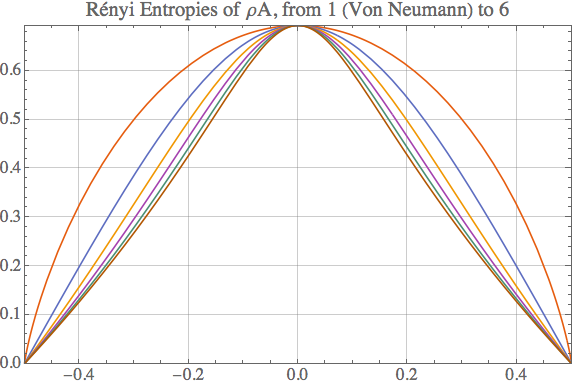
\includegraphics[width=0.8\textwidth]{Landi5_plot.png}
    \caption{Here are the plot of the computed entropies, in terms of the product \(cd\), which we know is bounded by \(\pm0.5\). As \(\alpha\) grows, the curves become sharper, meaning that the outermost curve is of Von Neumann's entropy, and the innermost curve is of \(\alpha=6\).}
    \label{fig:entropiesplot}
\end{figure}

It's good to see that the values for which \(S=0\) are exactly the points for which  \(\mathcal{P}_A=1\), \(cd=\pm1/2\). Also, the value of \(cd\) for which the entropy is maximum is simply \(c=0\) or \(d=0\), which implies that \(cd=0\). Using the result \eqref{eq:purA} we find that when the entropy is \(0\) the purity is \(1/2\), which is precisely \(1/n\) where \(n\) is the dimension of a qubit.


































































































































































































































































\chapter{Entangling through interactions}
\section{(a)} 
Unitary evolution means that the each state \(\ket{\psi_i}\) of the system undergoes \emph{individually} a unitary transformation, say, by the unitary operator \(U\). If
\begin{equation}
    \ket{\psi_i} \to U\ket{\psi_i},
\end{equation}
then
\begin{equation}
    \rho = \sum_i q_i \ketbra{\psi_i} \to \rho' = \sum_i U\ketbra{\psi_i}U^\dagger = U\rho U^\dagger.
\end{equation}
Carrying this transformation to \(\rho^2\) we find that
\begin{equation}
    \rho^2 \to \rho'^2 = \rho'\rho' = U\rho U^\dagger U \rho U^\dagger = U\rho^2 U^\dagger.
\end{equation}
Since the purity is defined as \(\mathcal{P} = \Tr(\rho^2)\), we can compute \(\mathcal{P}' = \Tr(\rho'^2)\):
\begin{equation}
    \mathcal{P} = \Tr(\rho'^2) = \Tr(U\rho^2 U^\dagger) \teq{Cyclic} \Tr(U^\dagger U\rho^2) = \Tr(\rho^2) = \mathcal{P}',
\end{equation}
and conclude that \(\mathcal{P} = \mathcal{P}'\), meaning that purity is preserved by any unitary evolution.

Also, since we can parameterise the purity by Bloch's vector \(\bm{s}\) as
\begin{equation}
    \mathcal{P} = \frac{1}{2}(1+\bm{s}^2)
\end{equation}
and \(\mathcal{P} = \mathcal{P}'\), we conclude that
\begin{equation}
    \bm{s}^2 = \bm{s'}^2 \qq{thus} \abs{\bm{s}} = \abs{\bm{s'}}.
\end{equation}
Since \(\bm{s} = r(\sin\theta\cos\phi,\sin\theta\sin\phi,\cos\theta)\), we see that
\begin{equation}
    r = r',
\end{equation}
thus any unitary evolution keeps states within the same shell of initial radius \(r\).

\section{(b)} 
First lets compute the Hamiltonian \(H = g(\sigma_{+}^1\sigma{-}^2 + \sigma_{-}^2\sigma_{+}^2)\):
\begin{equation}
    H = \mqty(0 & 0 & 0 & 0 \\ 0 & 0 & g & 0 \\ 0 & g & 0 & 0 \\ 0 & 0 & 0 & 0).
\end{equation}
Then, lets compute (using mathematica) the time-shift operator \(U = \exp{-iHt}\):
\begin{equation}
    U = \mqty(1 & 0 & 0 & 0 \\ 0 & \cos(gt) & -i\sin(gt) & 0 \\ 0 & -i\sin(gt) & \cos(gt) & 0 \\ 0 & 0 & 0 & 1).
\end{equation}

Since
\begin{equation}
    \ket{\psi(0)} = \ket{0,1}_{AB} = \mqty(0 \\ 1 \\ 0 \\ 0),
\end{equation}
we find that
\begin{equation}
    \ket{\psi(t)} = U \ket{\psi(0)} = \mqty(0 \\ \cos(gt) \\ -i\sin(gt) \\ 0) = \cos(gt)\ket{0,1} -i\sin(gt)\ket{1,0}.
\end{equation}

\section{(c)} 
Since
\begin{equation}
    \ket{\psi(t)} = \cos(gt)\ket{0,1} -i\sin(gt)\ket{1,0},
\end{equation}
we can compute \(\rho_{AB}\) as
\begin{equation}
\begin{split}
    \rho_{AB} = \ketbra{\psi(t)} = \cos^2(gt)&\ketbra{0,1} + i\sin(gt)\cos(gt)\ketbra{0,1}{1,0} +\\
    &- i\sin(gt)\cos(gt)\ketbra{1,0}{0,1} + \sin^2(gt)\ketbra{10},
\end{split}
\end{equation}
and take the partial trace over \(A\) and \(B\) to find the reduced density matrices
\begin{equation}\label{eq:rdmAB}
\begin{split}
    \rho_A &= \cos^2(gt)\ketbra{0} + \sin^2(gt)\ketbra{1} = \mqty(\cos^2(gt) & 0 \\ 0 & \sin^2(gt)), \\
    \rho_B &= \sin^2(gt)\ketbra{0} + \cos^2(gt)\ketbra{1} = \mqty(\sin^2(gt) & 0 \\ 0 & \cos^2(gt)).
\end{split}
\end{equation}
Since any qubit density matrix can be written as
\begin{equation}
    \rho(t) = \mqty(p(t) & \alpha(t) \\ \alpha^*(t) & 1-p(t))
\end{equation}
we readily identity
\begin{equation}
    p_A(t) = \cos^2(gt) \qand p_B(t) = \sin^2(gt)
\end{equation}
as the respective populations of \(A\) and \(B\).

\section{(d)}

Since the purity is defined as \(\mathcal{P} = \Tr(\rho^2)\), its quite simple to compute \(\mathcal{P}_A\) and \(\mathcal{P}_B\) from our previous results, namely \eqref{eq:rdmAB}:
\begin{equation}
\begin{split}
    \mathcal{P}_A(t) &= \cos^2(gt) + \sin^4(gt) \\
    \mathcal{P}_B(t) &= \sin^4(gt) + \cos^4(gt) = \mathcal{P}_A(t)
\end{split}
\end{equation}
\begin{figure}
    \centering
    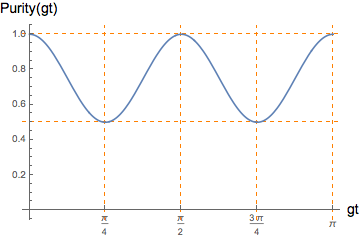
\includegraphics[width=0.8\textwidth]{QINFO_L01_06_Purity_Plot}
    \caption{Caption}
    \label{fig:purityplot}
\end{figure}

The figure \ref{fig:purityplot} shows us that the purity oscillates, meaning that, as time passes, the system becomes entangled and then after some time it becomes pure again. Since the purity is at its minimum when \(gt\) is an even multiple of \(\pi/4\), this is when the entanglement is at its maximum.

\section{(e)} 
Since
\begin{equation}
    \rho_A = \mqty(\cos^2(gt) & 0 \\ 0 & \sin^2(gt)),
\end{equation}
by Bloch's vector's parameterisation
\begin{equation}
    \rho = \frac{1}{2}\mqty(1+s_z & s_x - i s_y \\ s_x + i s_y & 1- s_z)
\end{equation}
we can readily identity
\begin{equation}
    \cos^2(gt) = \frac{1+s_z}{2} \qand s_x=s_y=0,
\end{equation}
and since
\begin{equation}
    s_z = 2\cos^2(gt) - 1 = \cos(2gt),
\end{equation}
we find that
\begin{equation}
    \bm{s} = (0,0,\cos(2gt)) = \cos(2gt) \mqty(0 & 0 & 1),
\end{equation}
thus \(r = \cos(2gt)\) and
\begin{equation}
\begin{split}
    \sin\theta\cos\phi = 0 \\
    \sin\theta\sin\phi = 0 \\
    \cos\theta = 1
\end{split}
\end{equation}
which can be solved only by \(\theta = 0\), for any \(\phi\). This means that, on Bloch's sphere, the qubit \(A\) simply oscillates along the \(z\)-axis, from the top \(r=1\), \(\ket{0}\), to the origin \(r=0\) and then to the bottom \(r=1\), \(\ket{1}\), and up again up to \(\ket{0}\).






































































































































































\chapter{Consuming correlations to reverse the flow of heat}

Consider two qubits with individual Hamiltonians \(H_A = -\Omega \sigma_z^A/2\) and \(H_B = -\Omega \sigma_z^B/2\). Suppose that they are initially prepared in a correlated state \begin{equation}
    \rho_{AB}(0) = \rho_A^0 \tens \rho_B^0 + \chi,
\end{equation}
where \(\rho_i^0 = \exp{-\beta_i H_i}/Z_i\), \(Z_i = \Tr(\exp{-\beta_i H_i})\) and \(\beta_i=1/T_i\). Also,
\begin{equation}
    \chi = \alpha (\ketbra{0,1}{1,0} + \ketbra{1,0}{0,1}),
\end{equation}
where \(\alpha\) is a constant. Lets subject the whole system to the Hamiltonian
\begin{equation}
    H = g(\sigma_x^A\sigma_y^B - \sigma_y^A\sigma_x^B).
\end{equation}

To find \(\rho_{AB}(t)\) we need to compute the time-shift operator \(U\), defined as
\begin{equation}
    U(t)=\exp{iHt}.
\end{equation}
Then
\begin{equation}
    \rho_{AB}(t)=U(t) \rho_{AB}(0) U^\dagger (t).
\end{equation}
Taking the partial trace over \(B\) of \(\rho_{AB}(t)\) we find
\begin{equation}
    \rho_A(t) = \Tr_B(\rho_{AB}(t)).
\end{equation}
The, to find \(\ev{H_A}\) we do
\begin{equation}
    E_A = \ev{H_A} = \Tr(H_A \rho_A(t)),
\end{equation}
and to find its derivative we simply do
\begin{equation}\label{eq:dHA}
    \dv{E_A}{t} = \dv{t}\Tr(H_A \rho_A(t)).
\end{equation}

To ease interpretation, let \(T_A = 1/\beta_A\) and \(T_B = 1/\beta_B\). Also, let \(\Omega = 1\) and \(g=1\). Having set \(T_A=0.3\) and \(T_B=0.4\), I plotted \eqref{eq:dHA} using Mathematica and obtained figure \ref{fig:dHA}.

\begin{figure}[H]
    \centering
    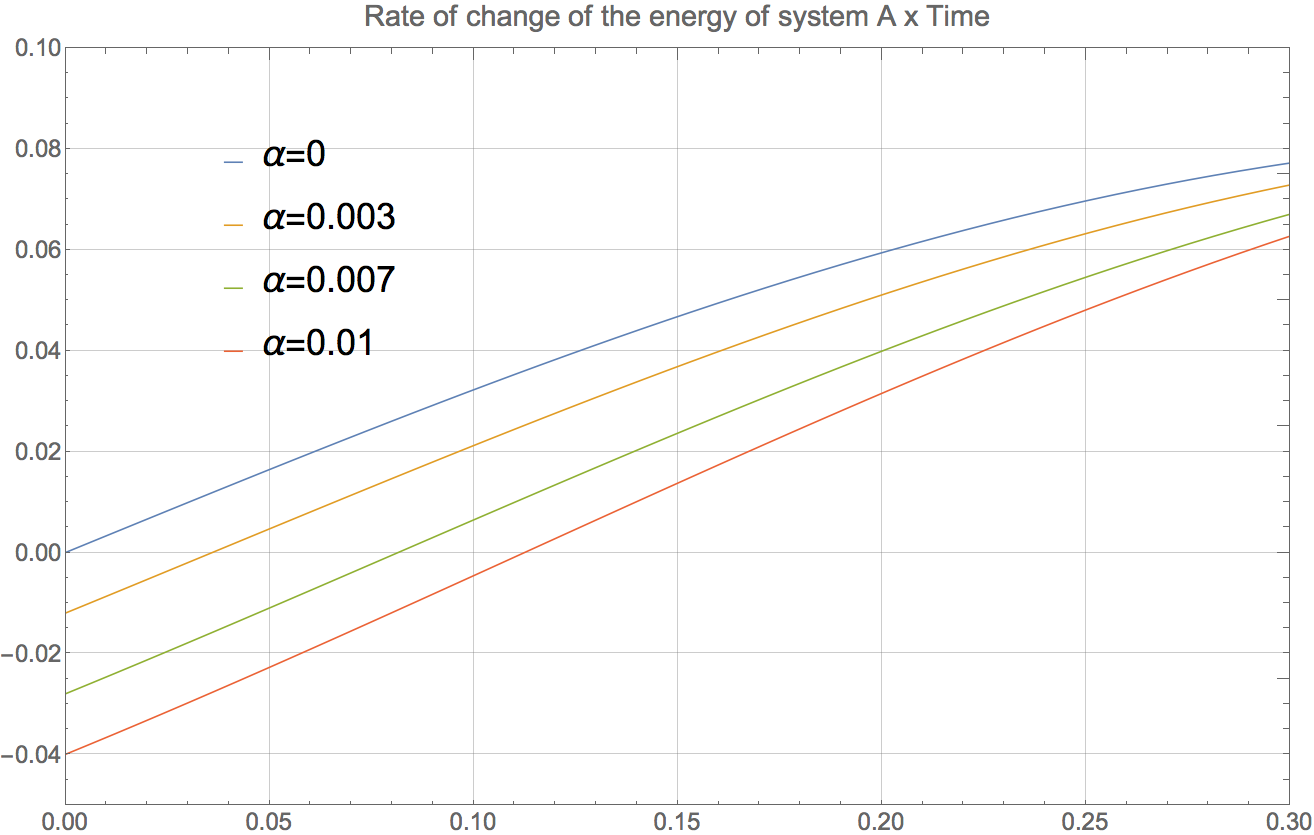
\includegraphics[width=\textwidth]{Landi7_dHA.png}
    \caption{Plot of \(\dv{\ev{H_A}}{t}\) by time, from \(t=0\) to \(t=0.3s\), with different correlation parameters \(\alpha\). At \(t=0\), system A is cooler than system B.}
    \label{fig:dHA}
\end{figure}

First of all recall that at \(t=0\) system \(A\) is cooler, so, classically, we expect system \(B\) to give energy to \(A\), thus we expect \(E_A\) to simply increase. From \ref{fig:dHA} we see that if the system has \(\alpha=0\), then \(E_A\) increases from the start of the interaction. However, as we increase \(\alpha\), we see that for some small amount of time the energy \(E_A\) actually \emph{decreases} before increases again. The stronger the correlation \(\alpha\) the longer system \(A\) loses energy before gaining it again. 

Another relevant thing to plot is the mutual information \(I_{AB}\), defined as
\begin{equation}\label{eq:mutINFO}
    I_{AB} = S(\rho_A) + S(\rho_A) - S(\rho_{AB}),
\end{equation}
where \(S\) denotes the Von Neumann entropy. We already know that all we need to compute entropies is the eigenvalues of the density matrices. Plotting \eqref{eq:mutINFO} we obtain figure \ref{fig:mutINFO}.

\begin{figure}[H]
    \centering
    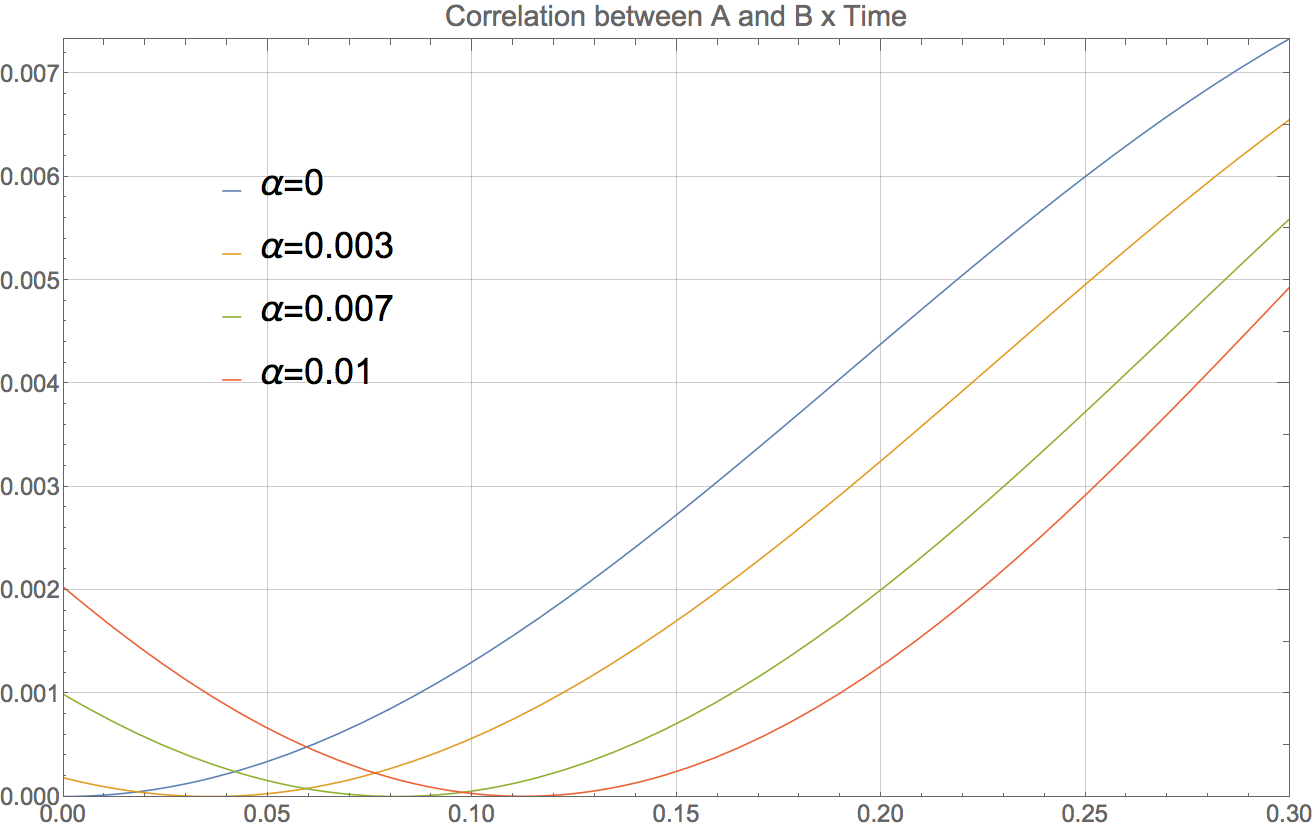
\includegraphics[width=\textwidth]{Landi7_Corr.png}
    \caption{Plot of \(I_{AB}\) by time, from \(t=0\) to \(t=0.3s\), with different correlation parameters \(\alpha\). At \(t=0\), system A is cooler than system B.}
    \label{fig:mutINFO}
\end{figure}

If there is no correlation \(\alpha\), then the mutual information at \(t=0\) is simply \(0\), as expected. Note that as \(\alpha\) increases the mutual information becomes larger at \(t=0\), meaning that the systems share information before interacting. However, as time passes the initial mutual information is lost, and then, of course, gained since the system interacts. It's important to see that \(I_{AB}\) becomes \(0\) exactly when \(\dv*{E_A}{t}\) changes sign, as we can see on figure \ref{fig:mutDHA}, which can be interpreted as the system consumes the initial mutual information in order to let the heat flow from the cold system \(A\) to the hotter system \(B\). However, after this initial mutual information is consumed, the systems behave like expected: heat goes from \(B\) to \(A\), hence \(E_A\) increases.

\begin{figure}
    \centering
    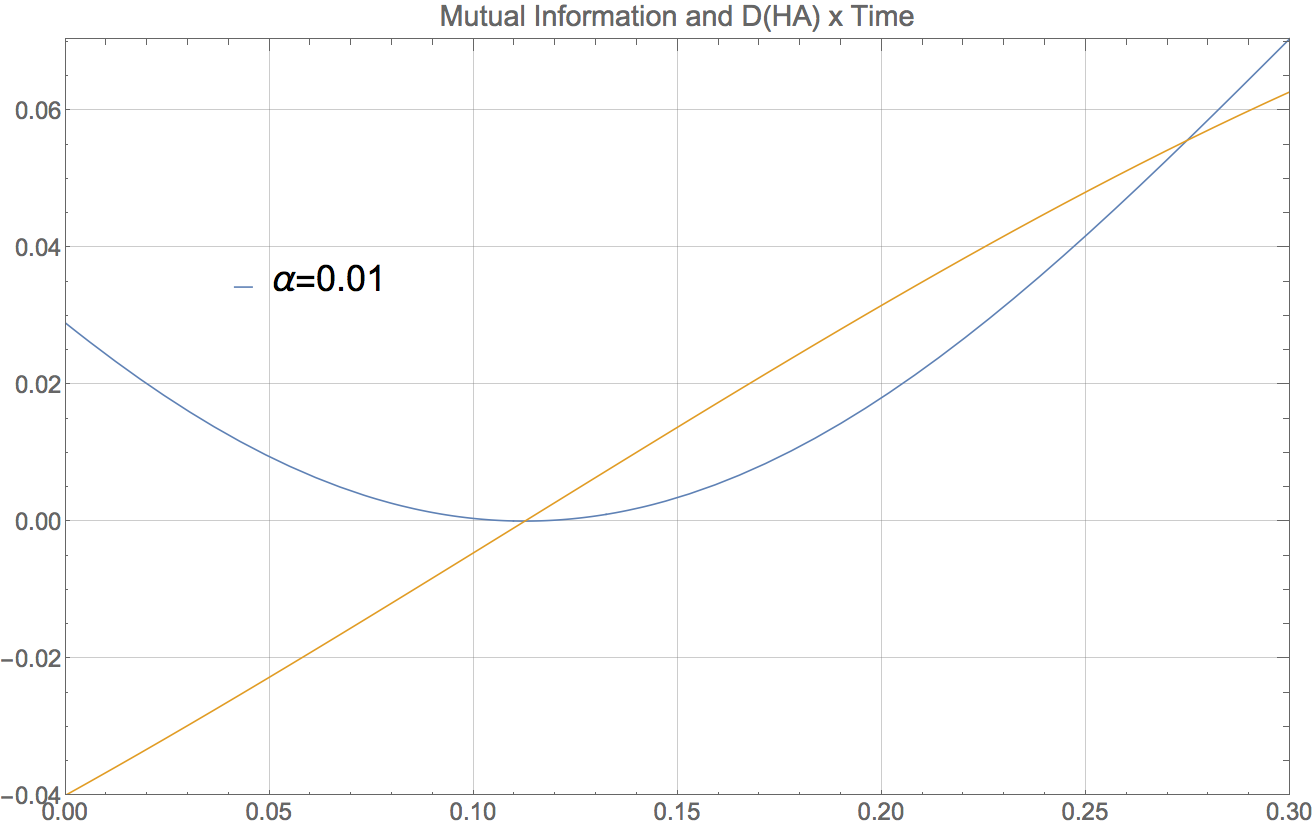
\includegraphics[width=\textwidth]{Landi7_MutDHA.png}
    \caption{Res-calling the previous plots to better compare them, we see that, for \(\alpha=0.01\), the energy \(E_A\) start to increase exactly when the initial mutual information is completely lost.}
    \label{fig:mutDHA}
\end{figure}




































% \backmatter
% \printbib
\end{document}